\PassOptionsToPackage{table}{xcolor}
\documentclass[10pt]{beamer}
\usepackage[english]{babel}

\usetheme{metropolis}
\usepackage{smartdiagram}
\usepackage{listings}
\usepackage{booktabs}
\usepackage[scale=2]{ccicons}%creative commons
\setbeamercovered{transparent}%invisible by default
\usepackage{array}
\newcolumntype{L}[1]{>{\raggedright\let\newline\\\arraybackslash\hspace{0pt}}m{#1}}
\newcolumntype{C}[1]{>{\centering\let\newline\\\arraybackslash\hspace{0pt}}m{#1}}
\newcolumntype{R}[1]{>{\raggedleft\let\newline\\\arraybackslash\hspace{0pt}}m{#1}}

\usepackage{pgfplots}
\usepgfplotslibrary{dateplot}
\usepackage{tikz}
\usepackage{tikz-uml}
\usetikzlibrary{positioning,chains,fit,shapes,calc,automata,positioning}
\newcommand{\mycomment}[1]{}
\usepackage{fancyvrb}
\usepackage{ifpdf}                        % To check if pdflatex is used.

\ifpdf
  \DeclareGraphicsRule{*}{mps}{*}{}       % To include metapost files.
\fi
% *****************************************************************************
% Matematica 
% *****************************************************************************

%\usepackage{amssymb}
%\usepackage{mathtools}                    % Add support for cramped,
					  
%\usepackage[euler]{flexisym}
%\usepackage{breqn}                        % Breqn
%\makeatletter
%   \def\eqnumsize{\normalfont \Tf@font}      % Add support to Minion Pro
%\makeatother
%\setkeys{breqn}{labelprefix={eq:}}


%\usepackage{asymptote}
%\usepackage[loop, controls]{animate}

\graphicspath{{./}, {./Images/}}

\lstdefinelanguage{Kotlin}{
  keywords={package, as, typealias, this, super, val, var, fun, for, null, true, false, is, in, throw, return, break, continue, object, if, try, else, while, do, when, yield, typeof, yield, typeof, class, interface, enum, object, override, public, private, get, set, import, abstract, },
  keywordstyle=\color{blue}\bfseries,
  ndkeywords={@Deprecated, Int, Integer, Float, Double, String, Runnable, dynamic},
  ndkeywordstyle=\color{red}\bfseries,
  emph={println, return@, forEach,},
  emphstyle={\color{red}},
  identifierstyle=\color{black},
  sensitive=true,
  commentstyle=\color{gray}\ttfamily,
  comment=[l]{//},
  morecomment=[s]{/*}{*/},
  stringstyle=\color{gray}\ttfamily,
  morestring=[b]",
  morestring=[s]{"""*}{*"""},
}

\providecommand{\ie}{i.\,e.}
\providecommand{\Ie}{I.\,e.}
\providecommand{\eg}{e.\,g.}
\providecommand{\Eg}{E.\,g.} 

\metroset{block=fill}
\metroset{titleformat frame=smallcaps}

\title{Having fun with Kotlin coroutines}
%\subtitle{Ariadne's thread in Kotlin models of concurrency}
\subtitle{A first tour of concurrency models in Kotlin}

\date{\today}
\author[A. Candolini]{Alessandro Candolini}
%\institute{Department of Physics, University of Trieste}
% \titlegraphic{\hfill\includegraphics[height=1.5cm]{logo/logo}}

\begin{document}

\maketitle

\begin{frame}{Agenda}
  \setbeamertemplate{section in toc}[sections numbered]
  \tableofcontents[hideallsubsections]
\end{frame}

\section{We live in a concurrent world}
\begin{frame}[fragile]
	\begin{figure}
		\centering
		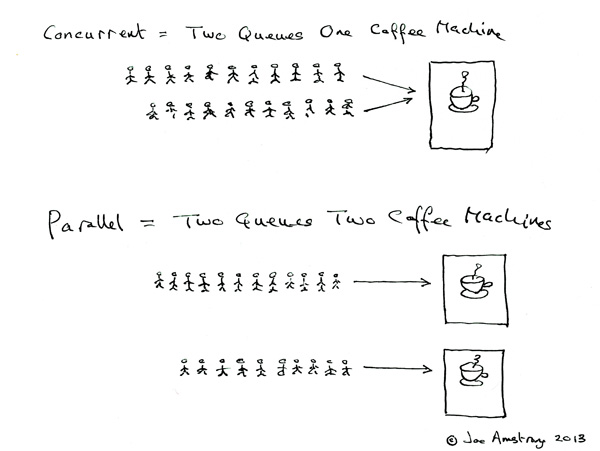
\includegraphics[width=.8\textwidth]{concurrency_coffee}
		\caption{\url{https://joearms.github.io/published/2013-04-05-concurrent-and-parallel-programming.html}}
	\end{figure}
\end{frame}
\begin{frame}[fragile]
Is concurrency relevant for mobile development?
	\begin{itemize} 
		\item<2-> IO (\eg, network, etc) 
		\item<3-> sensors (\eg, gps, etc) 
		\item<4-> UI events 
		\item<5-> platform lifecycle 
	\end{itemize}
\end{frame}
\begin{frame}[fragile]
\begin{columns}
\begin{column}{0.4\textwidth}
	\begin{center}
	\begin{figure}
		\centering
		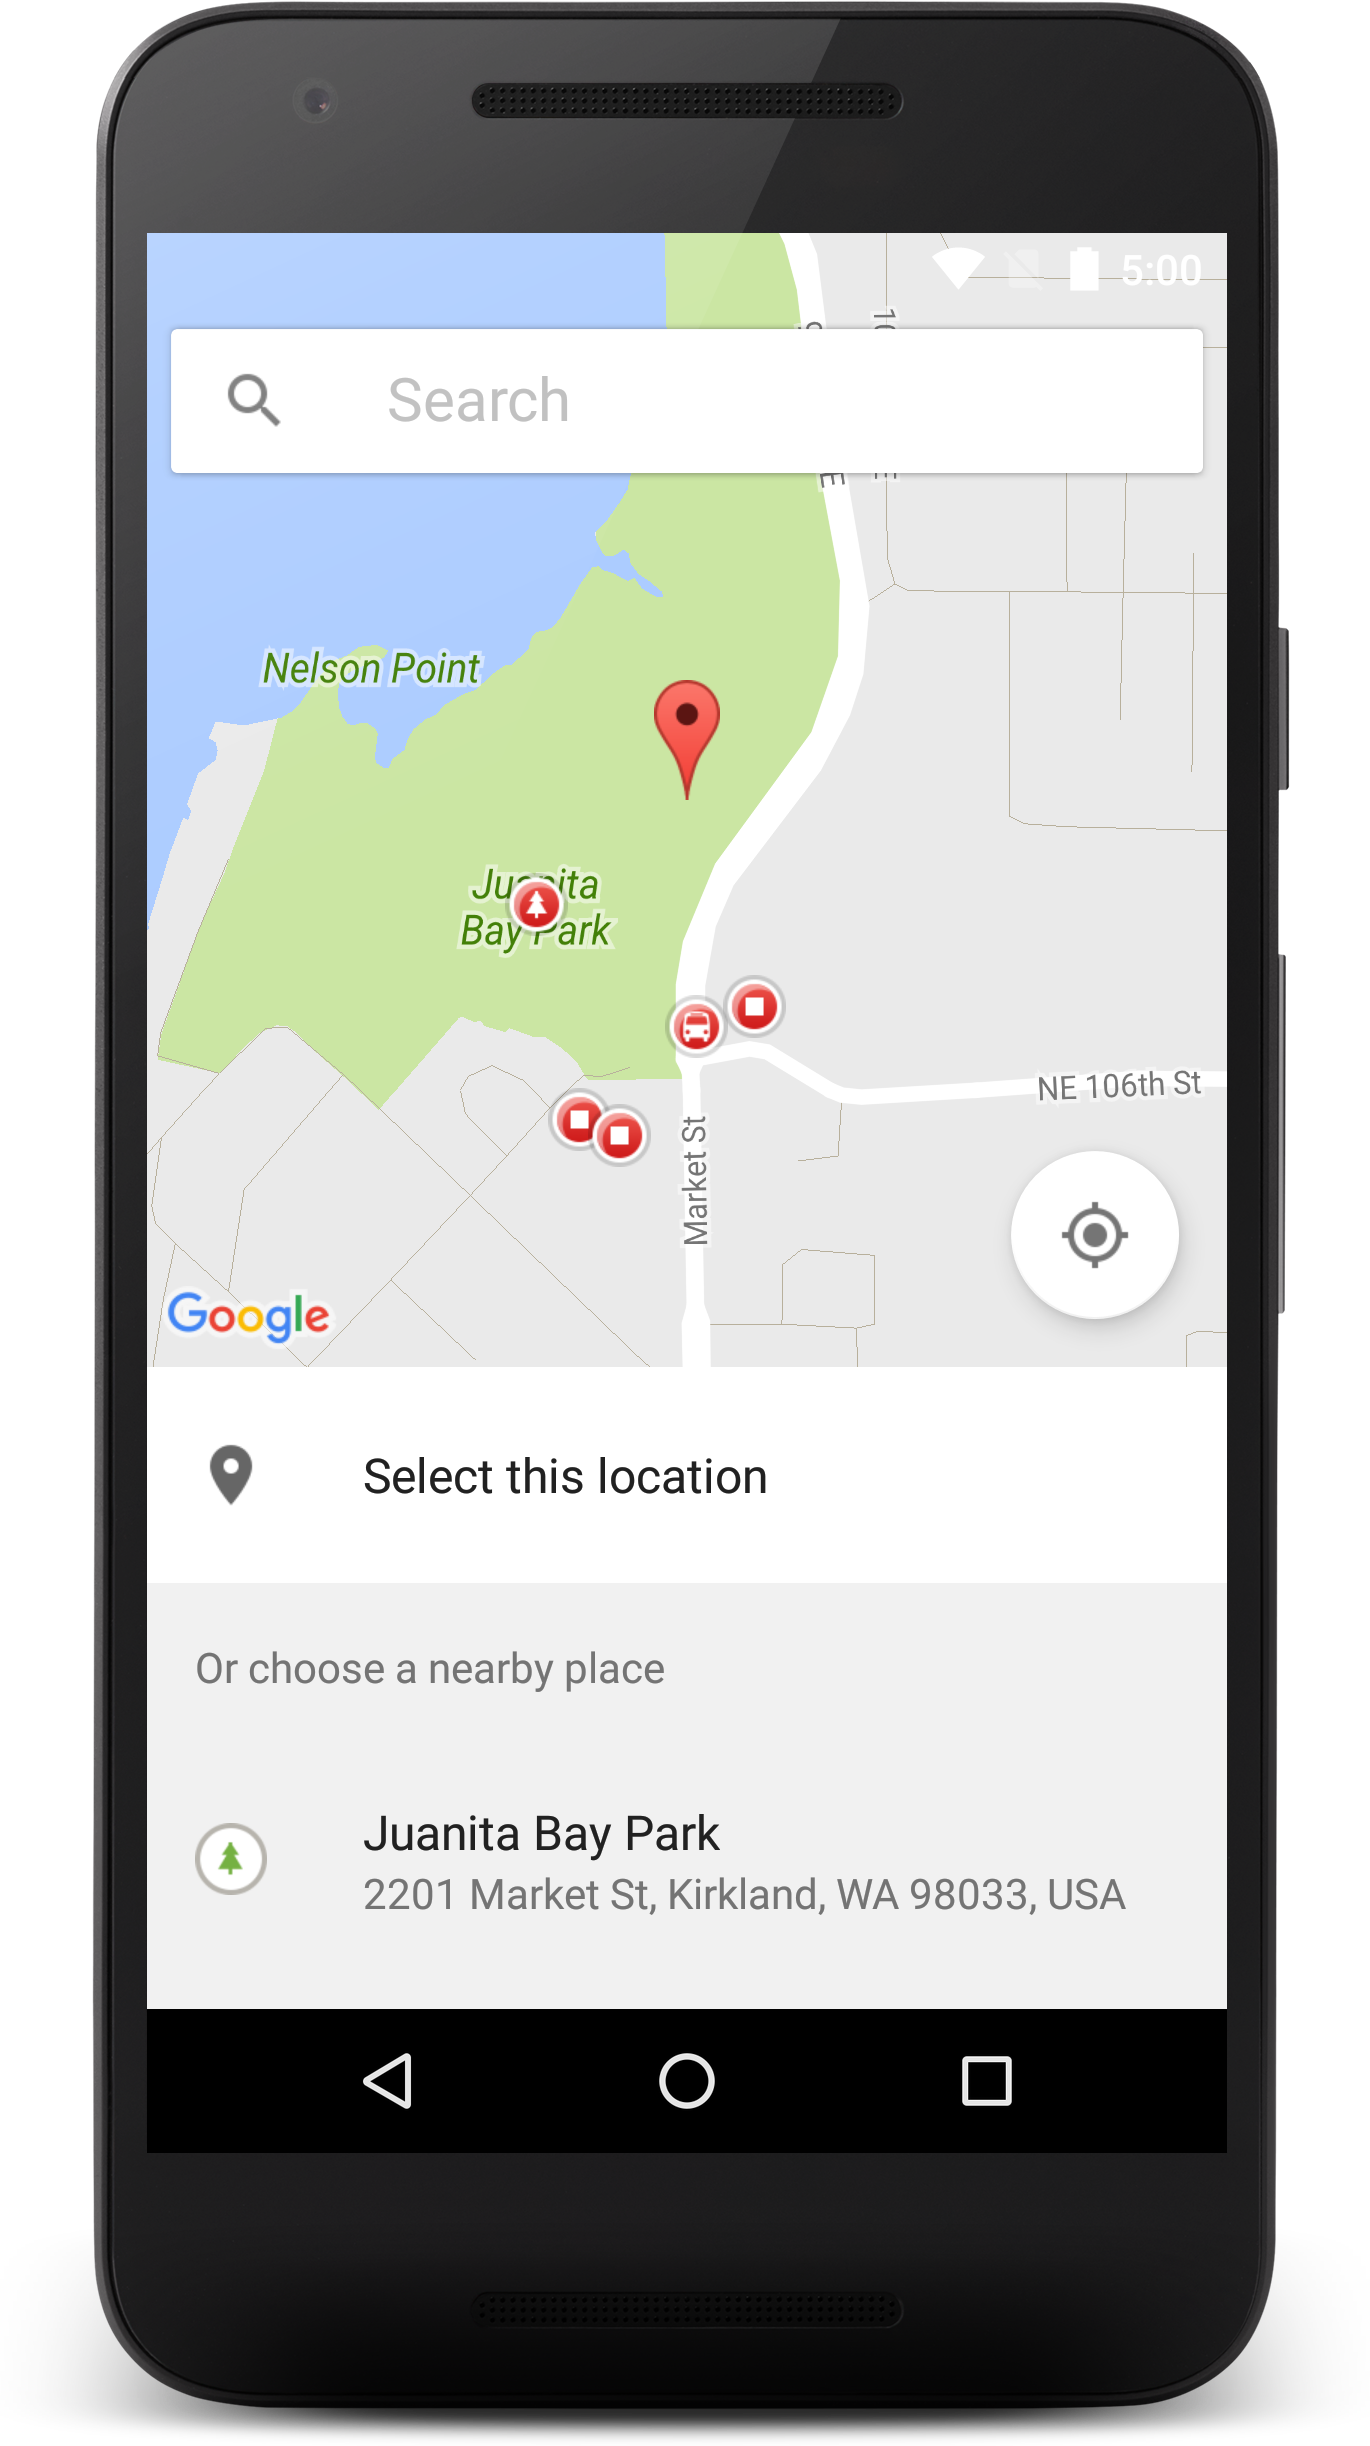
\includegraphics[height=.8\textheight]{location}
	\end{figure}
	\end{center}
\end{column}
\begin{column}{0.6\textwidth}
	acceptance criteria:
	\begin{itemize}
		\item search by current location 
		\item search by location name 
	\end{itemize}
	advanced 
	\begin{itemize}
		\item search suggestions when tying 
	\end{itemize}
\end{column}
\end{columns}
\end{frame}
\begin{frame}[fragile]
	Translate ACs into code: simple \emph{sequential} state machine  (simplified) 
	\begin{figure}
		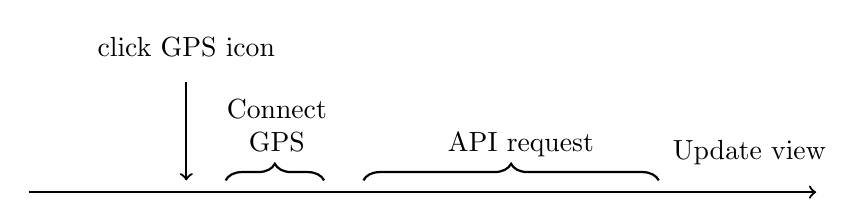
\begin{tikzpicture}[scale=1]
%\node[align=center] at (1,0.5) {Enter};
\node[align=center] at (2,1.85) {click GPS icon};
\draw [thick,->] (2,1.4) -- (2,0.15);
\node[align=center] at (3.15,0.85) {Connect\\GPS};
\draw [thick,decorate,decoration={brace,amplitude=6pt,raise=0pt}] (2.5,0.15) -- (3.75,0.15);
%\draw [thick,->] (4,0.85) -- (4,0.15);
\node[align=center] at (6.25,0.6) {API request};
%\draw [thick,->] (8.25,0.85) -- (8.25,0.15);
\node[align=center] at (9.15,0.5) {Update view};
\draw [thick,decorate,decoration={brace,amplitude=6pt,raise=0pt}] (4.25,0.15) -- (8,0.15);
\draw [thick,->] (0,0) -- (10,0);
%\draw [thick,->] (4.6,-0.85) -- (4.6,-0.15);
%\draw [thick,->] (7.65,-0.4) -- (7.65,-0.15);
%\draw [thick,decorate,decoration={brace,amplitude=6pt,raise=0pt,mirror}] (4.75,-0.15) -- (7.5,-0.15);
%\node[align=center] at (6.25,-0.85) {Symptomatic\\period};
%\node[align=center] at (4.6,-1.3) {Onset of\\symptoms};
\end{tikzpicture}
	\end{figure}
\begin{figure}
		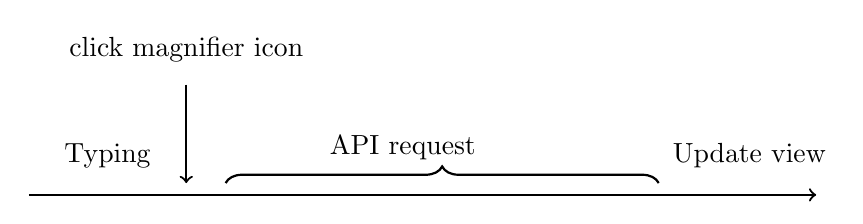
\begin{tikzpicture}[scale=1]
\node[align=center] at (1,0.5) {Typing};
\node[align=center] at (2,1.85) {click magnifier icon};
\draw [thick,->] (2,1.4) -- (2,0.15);
%\node[align=center] at (3.15,0.85) {Connect\\GPS};
%\draw [thick,decorate,decoration={brace,amplitude=6pt,raise=0pt}] (2.5,0.15) -- (3.75,0.15);
%\draw [thick,->] (4,0.85) -- (4,0.15);
\node[align=center] at (4.75,0.6) {API request};
%\draw [thick,->] (8.25,0.85) -- (8.25,0.15);
\node[align=center] at (9.15,0.5) {Update view};
\draw [thick,decorate,decoration={brace,amplitude=6pt,raise=0pt}] (2.5,0.15) -- (8,0.15);
\draw [thick,->] (0,0) -- (10,0);
%\draw [thick,->] (4.6,-0.85) -- (4.6,-0.15);
%\draw [thick,->] (7.65,-0.4) -- (7.65,-0.15);
%\draw [thick,decorate,decoration={brace,amplitude=6pt,raise=0pt,mirror}] (4.75,-0.15) -- (7.5,-0.15);
%\node[align=center] at (6.25,-0.85) {Symptomatic\\period};
%\node[align=center] at (4.6,-1.3) {Onset of\\symptoms};
\end{tikzpicture}
	\end{figure}

\end{frame}
\begin{frame}[fragile]
	\begin{figure}
		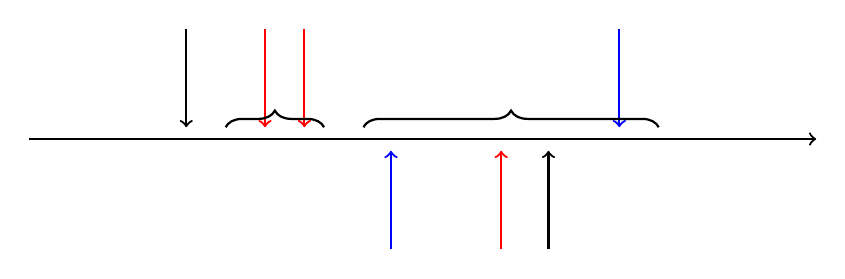
\begin{tikzpicture}[scale=1]
%\node[align=center] at (1,0.5) {Enter};
\draw [thick,->] (2,1.4) -- (2,0.15);
\draw [red, thick,->] (3,1.4) -- (3,0.15);
\draw [red, thick,->] (3.5,1.4) -- (3.5,0.15);
\draw [blue, thick,->] (7.5,1.4) -- (7.5,0.15);
\draw [blue, thick,->] (4.6,-1.4) -- (4.6,-0.15);
\draw [red, thick,->] (6.0,-1.4) -- (6.0,-0.15);
\draw [thick,->] (6.6,-1.4) -- (6.6,-0.15);
%\node[align=center] at (3.15,0.85) {Connect\\GPS};
\draw [thick,decorate,decoration={brace,amplitude=6pt,raise=0pt}] (2.5,0.15) -- (3.75,0.15);
%\draw [thick,->] (4,0.85) -- (4,0.15);
%\node[align=center] at (6.25,0.6) {API request};
%\draw [thick,->] (8.25,0.85) -- (8.25,0.15);
%\node[align=center] at (9.15,0.5) {Update view};
\draw [thick,decorate,decoration={brace,amplitude=6pt,raise=0pt}] (4.25,0.15) -- (8,0.15);
\draw [thick,->] (0,0) -- (10,0);
%\draw [thick,->] (4.6,-0.85) -- (4.6,-0.15);
%\draw [thick,->] (7.65,-0.4) -- (7.65,-0.15);
%\draw [thick,decorate,decoration={brace,amplitude=6pt,raise=0pt,mirror}] (4.75,-0.15) -- (7.5,-0.15);
%\node[align=center] at (6.25,-0.85) {Symptomatic\\period};
%\node[align=center] at (4.6,-1.3) {Onset of\\symptoms};
\end{tikzpicture}
	\end{figure}
\end{frame}



\begin{frame}[fragile]
\begin{columns}
\begin{column}{0.5\textwidth}
	\begin{center}
	\begin{figure}
		\centering
		
\includegraphics[height=.6\textheight]{tip}
	\end{figure}
	\end{center}
\end{column}
\begin{column}{0.6\textwidth}
	\begin{itemize}
		\item Delays
		\item User inputs 
		\item Failures (connectivity, gps on mobile devices)
		\item Ordering of api response
		\item \emph{android/ios lifecycle}, etc
	\end{itemize}
\end{column}
\end{columns}

\end{frame}

\begin{frame}[fragile]
	\begin{figure}
		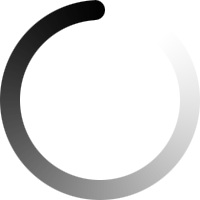
\includegraphics[width=.7\textwidth]{loading}
	\end{figure}
\end{frame}
\begin{frame}[fragile]
	First approach: put constrains in place to restrict the range of possible options  
	\begin{itemize}
		\item Conditionally forbid user events (disable buttons, loading spinners, etc) 
		\item Boolean flags 
		\item Be defensive (if/else) 
		\item Bind/unbind from lifecycle , etc
	\end{itemize}
	(Or more technical constrains like single thread executors, queues, synchronization, etc)
\end{frame}

\begin{frame}
	The approach doesn't scale. 

	\begin{itemize}
		\item Pre-fatching
		\item Background upload
		\item Recovery/retry logic 
		\item debouncing, timeouts 
		\item no control on platform lifecycle
	\end{itemize}

\end{frame}

\begin{frame}[fragile]
	``Concurrency is the composition of independently executing processes, typically functions, but they don't have to be.''

	``Parallelism is the simultaneous execution of multiple things, possibly related, possibly not.''

Rob Pike

\end{frame}
\begin{frame}[fragile]
	\begin{figure}
		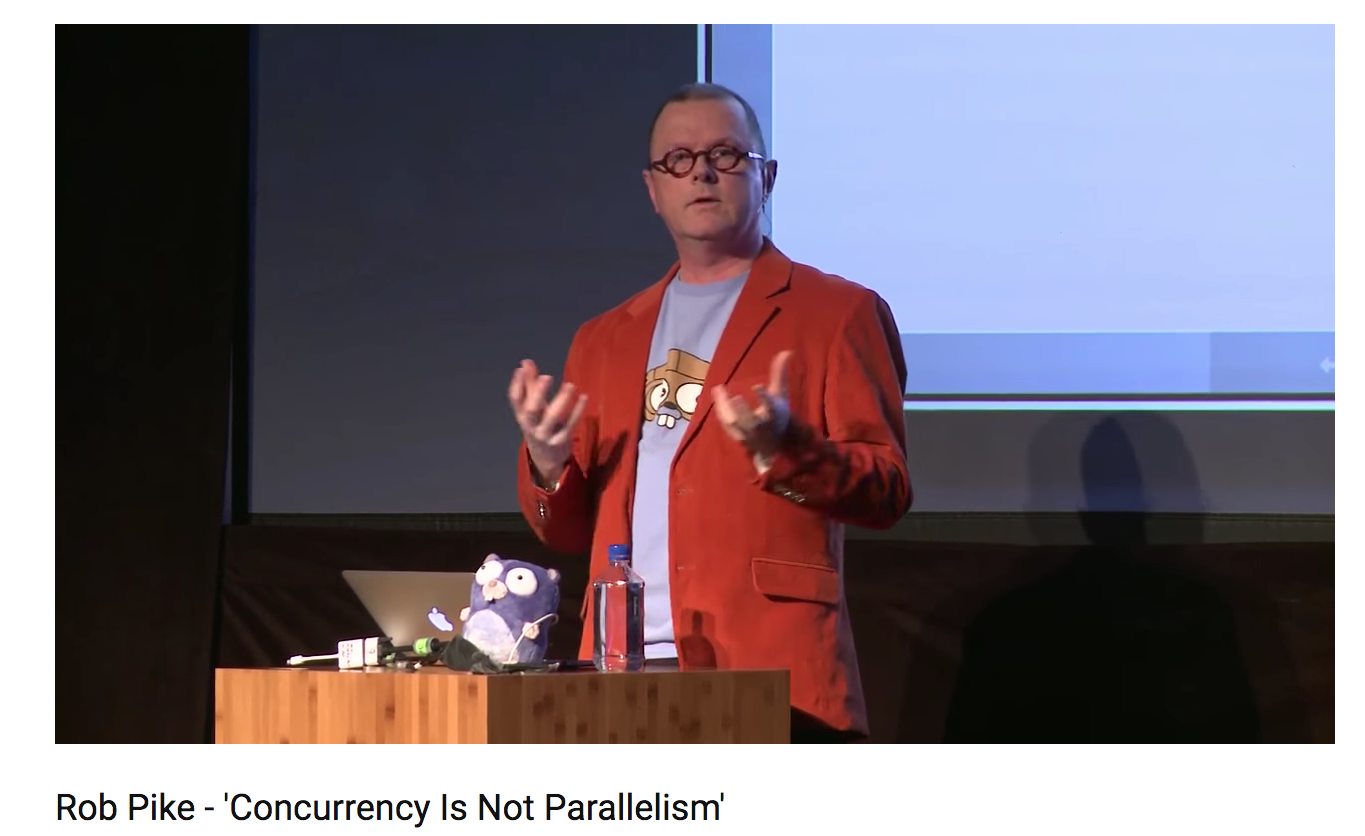
\includegraphics[height=.8\textheight]{rob_talk}
		\caption{\url{https://www.youtube.com/watch?v=cN_DpYBzKso&t=1061s}}
	\end{figure}
\end{frame}

\begin{frame}[fragile]
	\begin{figure}
		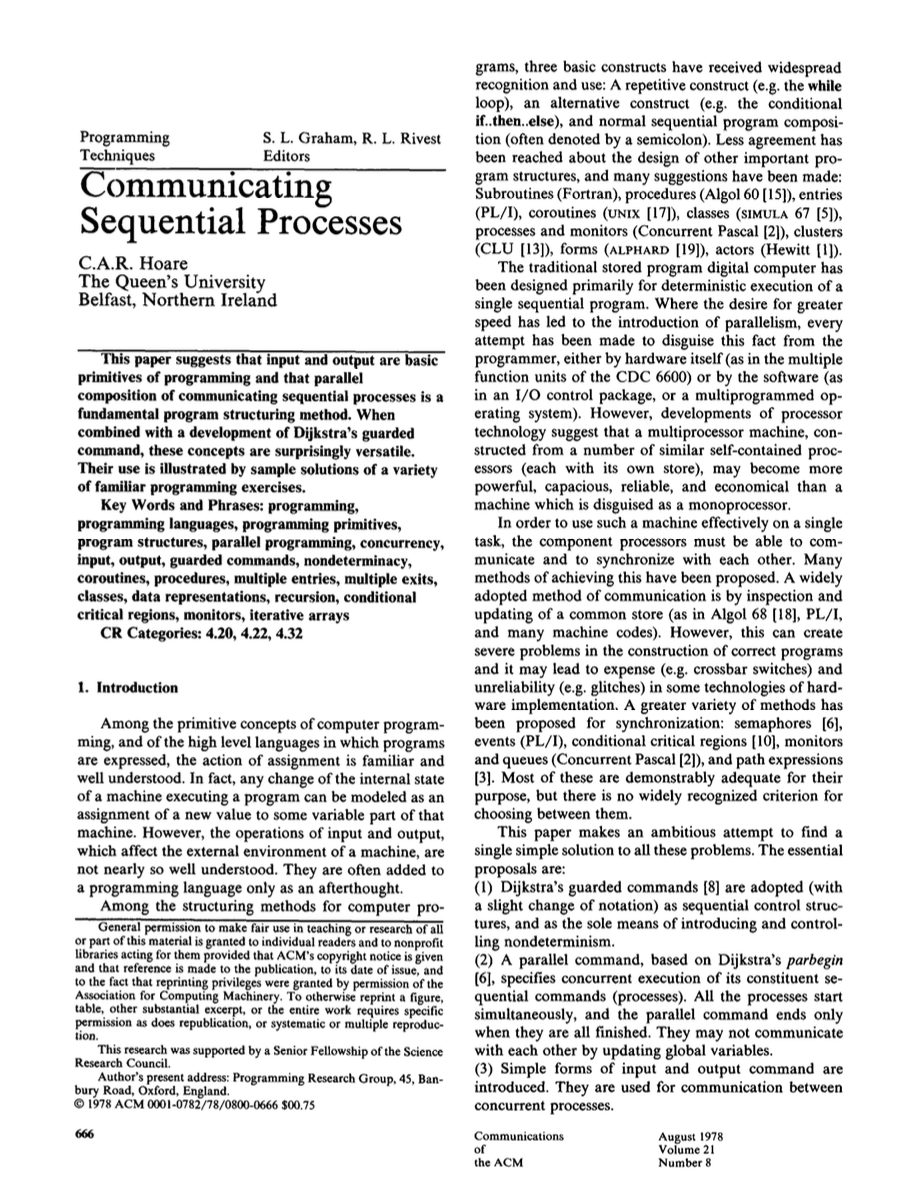
\includegraphics[height=.8\textheight]{tony}
		\caption{Tony Hoare's seminal paper}
	\end{figure}
\end{frame}
\begin{frame}[fragile]
``The most obvious application of the new ideas is to the specification, design,
and implementation of computer systems which continuously act and
interact with their environment. The basic idea is that these systems can be
readily decomposed into subsystems which operate concurrently and interact
with each other as well as with their common environment. The parallel composition
of subsystems is as simple as the sequential composition of lines or
statements in a conventional programming language.``

	Tony Hoare (CSP book, 2015)
\end{frame}



\begin{frame}[fragile]
Java definition of concurrency and Leslie Lamport seminal paper 
\end{frame}
\begin{frame}[fragile]
Traditional picture of concurrency vs parallelism: coffe machine 
\end{frame}
\begin{frame}[fragile]
Better reppresentation: driving in the desert vs driving in London 
	\begin{figure}
		\centering
		\includegraphics{car-1}\\
		\includegraphics{car-2}
	\end{figure}
\end{frame}
\begin{frame}[fragile]
The deep problem: \emph{communication}

	Communicating, orchestrating independent processing. Software development as a \emph{dialog} between parts. 

	We will just sketch the surface of this deeper problem by focusing only  on a smaller technical problem in this talk: \emph{blocking} and \emph{non wasting unnecessary resources when waiting}
\end{frame}
\section{Blocking vs non-blocking}
\begin{frame}
	Test
%\begin{lstlisting}[language=Kotlin, basicstyle=\ttfamily]
%\end{lstlisting}
\end{frame}
\section{Demystifying coroutines}
\begin{frame}
What rae
\end{frame}
\section{Coroutines-powered concurrency models}
\begin{frame}[fragile]
\begin{itemize}
	\item CSP (aka, channels) 
\item actors 
	\end{itemize}
\end{frame}
\plain{Questions?}

%\begin{frame}[allowframebreaks] {References}
% \bibliography{demo}
% \bibliographystyle{abbrv}
%\end{frame}

\end{document}
\begin{lstlisting}[language=Kotlin, basicstyle=\ttfamily]
\end{lstlisting}
